\chapter{Perancangan}
\label{chap:perancangan}

Pada bab ini akan dijelaskan mengenai perancangan perangkat lunak yang meliputi: perancangan proses visualisasi dan perancangan antarmuka

\section{Perancangan Proses Visualisasi}
Untuk Perancangan proses visualisai akan dijelaskan menggunakan flowchart diagram yang dilanjutkan dengan perancangan struktur aplikasi. 

\subsection{Flowchart Diagram}
Untuk diagaram alur aplikasi VisKur dapat dilihat pada Gambar \ref{fig:gambarFlowchart}.

\begin{figure}[H]
    \centering
    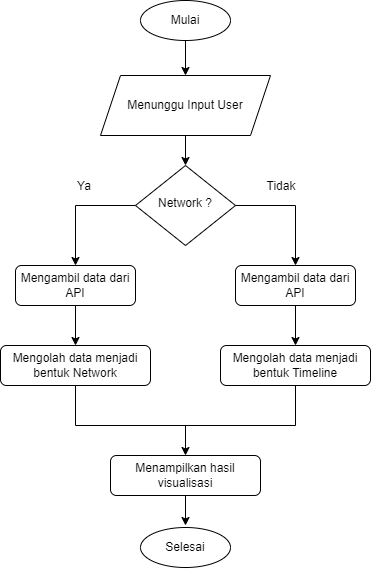
\includegraphics[width=8cm, height=12cm]{Gambar/flowchart.png}
    \caption{\textit{Flowchart} aplikasi VisKur}
    \label{fig:gambarFlowchart}
\end{figure}

\newpage
Saat pertama kali perangkat lunak dijalankan, perangkat lunak akan menunggu \textit{input user}, apakah pengguna akan meminta dibuatkan visualisasi kurikulum 2018 dalam bentuk \textit{Network} atau bentuk \textit{Timeline}. Jika pengguna memlih bentuk \textit{Network}, maka perangkat lunak akan segera mengambil data dari API, mengolah data tersebut menjadi bentuk \textit{Network}, dan ketika sudah selesai mengolahnya, maka perangkat lunak akan menampilkan hasil visualisasi dalam bentuk \textit{Network} tersebut. Jika pengguna tidak memilih bentuk \textit{Network} yang artinya memilih bentuk \textit{Timeline}, maka maka perangkat lunak akan segera mengambil data dari API, mengolah data tersebut menjadi bentuk \textit{Timeline}, dan ketika sudah selesai mengolahnya, makan perangkat lunak akan menampilkan hasil visualisasi dalam bentuk \textit{Timeline} tersebut. Ketika perangkat lunak sudah berhasil menampilkan hasil visualisai ke dalam bentuk yang diinginkan pengguna, maka perangkat lunak akan selesai.

\subsection{Perancangan Struktur Aplikasi}

Struktur aplikasi merupakan susunan direktori untuk membangun aplikasi tersebut. Struktur ini terdiri dari
berbagai folder dan berkas yang telah dipisahkan berdasarkan fungsinya masing-masing. Berikut ini merupakan penjelasan masing-masing folder dan berkas yang digunakan untuk membuat aplikasi VisKur:

\begin{itemize}
    \item \textbf{folder css}, folder ini berisi berkas - berkas dengan ekstensi \textit{css} yang digunakan untuk mengatur tampilan aplikasi. Terdapat berbagai berkas pada folder ini, yaitu:
    \begin{itemize}
        \item \textbf{vis-network.min.css}, berkas \textit{css} ini berfungsi untuk mengatur tampilan setiap elemen \textit{network} pada \textit{Vis.js}.
        \item \textbf{vis-timeline-graph2d.min.css},
        berkas \textit{css} ini berfungsi untuk mengatur tampilan setiap elemen \textit{timeline} pada \textit{Vis.js}.
        Pada berkas ini akan ditambahkan Kode \ref{lst:kodeCSSGraph2d} yang berfungsi untuk memberikan warna pada setiap \textit{content} yang ditampilkan.
        
        \begin{lstlisting}[language=JavaScript, caption=Tambahan kode \textit{vis-timeline-graph2d.min.css}\label{lst:kodeCSSGraph2d}]
        .vis-item.lightBlue {
          background-color: rgb(151, 194, 252);
          border-color: rgb(43, 124, 233);
          color: black;
          box-shadow: 0 0 10px gray;
        }
        .vis-item.yellow {
            background-color: rgb(255,255,0);
            border-color:rgb(255,165,0);
            color: black;
            box-shadow: 0 0 10px gray;
          }
        .vis-item.red {
          background-color: rgb(251,126,129);
          border-color: rgb(251,70,74);
          color: black;
          box-shadow: 0 0 10px gray;
        }
        .vis-item.green {
          background-color: rgb(123,225,65);
          border-color: rgb(76,177,19);
          color: black;
          box-shadow: 0 0 10px gray;
        }
        .vis-item.pink {
          background-color: rgb(235,125,244);
          border-color: rgb(225,41,240);
          color: black;
          box-shadow: 0 0 10px gray;
        }
        .vis-item.purple {
          background-color: rgb(173,133,228);
          border-color: rgb(124,41,240);
          color: black;
          box-shadow: 0 0 10px gray;
        }
        .vis-item.orange {
          background-color: rgb(255,168,7);
          border-color: rgb(217,142,3);
          color: black;
          box-shadow: 0 0 10px gray;
        }
        .vis-item.darkBlue {
          background-color: rgb(110,110,253);
          border-color: rgb(68,35,251);
          color: black;
          box-shadow: 0 0 10px gray;
        }
        \end{lstlisting}
        
        \item \textbf{vis.css}, berkas \textit{css} ini berfungsi untuk mengatur tampilan dan animasi untuk semua jenis visualisasi yang terdapat pada \textit{Vis.js}.
    \end{itemize}

    \item \textbf{folder js}, folder ini berisi berkas - berkas dengan ekstensi js. Terdapat berbagai berkas pada folder ini, yaitu:
    \begin{itemize}
        \item \textbf{network.js}, berkas \textit{JavaScript} ini berisi fungsi khusus untuk membuat visualisai dalam bentuk \textit{network}. Fungsi pada berkas ini nantinya akan dipanggil pada  index.html. Untuk kodenya dapat dilihat pada Kode \ref{lst:kodeNetworkJs}.
        
        \begin{lstlisting}[language=JavaScript, caption=Kode \textit{network.js}\label{lst:kodeNetworkJs}]
        function processNetwork (){
            document.getElementById("timeline").style.display="none"
            document.getElementById("network").style.display="inline"
            let matkul = '';
            const fetchUsers = async () => {
                try {
                    const res = await fetch('https://raw.githubusercontent.com/ftisunpar/data/master/prasyarat.json');
                    if (!res.ok) {
                        throw new Error(res.status);
                    }
                    const data = await res.json();
                    matkul = data;
                    createNetwork();
                } catch (error) {
                    console.log(error);
                }
            }
            
            var nodes = new vis.DataSet();
        
            var edges = new vis.DataSet();
        
            function createNetwork() {
                const horizontal = [];
                for (i = 1; i < 9; i++) {
                    nodes.add([{
                        id: i, label: "Semester " + i, group: i, y: i*150
                    }])
                    if (i != 8) {
                        edges.add([
                            { from: i, to: i + 1 }
                        ])
                    }
                    horizontal[i] = 0;
                }
                
                for (let i = 0; i < matkul.length; i++) {
                    let shape=""
                    if(matkul[i].wajib){
                        shape="box"
                    }
                    else{
                        shape="circle"
                    }
        
                    horizontal[matkul[i].semester] += 200; 
                    nodes.add([{
                        id: matkul[i].kode, label: matkul[i].nama, group: matkul[i].semester, 
                        x:horizontal[matkul[i].semester], y: matkul[i].semester*150, shape:shape 
                    }])
        
                    if(matkul[i].prasyarat.tempuh.length != 0){
                        for (let j = 0; j < matkul[i].prasyarat.tempuh.length; j++){
                            edges.add([
                                { from: matkul[i].kode, to: matkul[i].prasyarat.tempuh[j], 
                                  arrows: "from"}
                            ])
                        }
                    }
                    if(matkul[i].prasyarat.lulus.length != 0){
                        for (let j = 0; j < matkul[i].prasyarat.lulus.length; j++){
                            edges.add([
                                { from: matkul[i].kode, to: matkul[i].prasyarat.lulus[j], 
                                  dashes: true }
                            ])
                        }
                    }
                    if(matkul[i].prasyarat.bersamaan.length != 0){
                        for (let j = 0; j < matkul[i].prasyarat.bersamaan.length; j++){
                            edges.add([
                                { from: matkul[i].kode, to: matkul[i].prasyarat.bersamaan[j], 
                                  arrows: "from", dashes: true }
                            ])
                        }
                    }
                }
            }
            fetchUsers();
        
            var container = document.getElementById('network');
        
            var data = {
                nodes: nodes,
                edges: edges
            };
        
            var options = {
                nodes: {
                    margin: 10,
                    widthConstraint: {
                        maximum: 120,
                    },
                },
                physics: false,
                edges: {
                    smooth: false
                },
            };
            
            var network = new vis.Network(container, data, options);
        }
        \end{lstlisting}
        
        \item \textbf{timeline.js}, berkas \textit{JavaScript} ini berisi fungsi khusus untuk membuat visualisai dalam bentuk \textit{timeline}. Fungsi pada berkas ini nantinya akan dipanggil pada  index.html. Untuk kodenya dapat dilihat pada Kode \ref{lst:kodeTimelineJs}.
        
        \begin{lstlisting}[language=JavaScript, caption=Kode \textit{timeline.js}\label{lst:kodeTimelineJs}]
        function processTimeline(){
          document.getElementById("network").style.display="none"
          document.getElementById("timeline").style.display="inline"
          let matkul = ''
          const fetchUsers = async () => {
              try {
                  const res = await fetch('https://raw.githubusercontent.com/ftisunpar/data/master/prasyarat.json');
                  if (!res.ok) {
                      throw new Error(res.status);
                  }
                  const data = await res.json();
                  matkul = data;
                  createTimeline(matkul);
              } catch (error) {
                  console.log(error);
              }
          }
          
          function createTimeline() {
              var groups = new vis.DataSet([
                { id: 1, content: "Mata Kuliah Wajib" },
                { id: 2, content: "Mata Kuliah Pilihan" },
              ]);
        
              let tahun=new Date().getFullYear();
              let bulan = new Date().getMonth();
              if(bulan<7){
                tahun-=1
                bulan=7
              }
              else{
                bulan=7
              }
        
              let semester=[]
              for(i=1;i<=9;i++){
                  semester[i]= tahun.toString()+"-"+bulan.toString()+"- 31"
                  if(i%2!=0){
                    bulan+=5
                  }
                  else{
                    bulan-=5
                    tahun+=1
                  }
              }
        
              var res = [];
              let color=["","lightBlue","yellow","red","green","pink","purple","orange","darkBlue"]
              for (var i = 0; i < matkul.length; i++) {
                  let wajib=''
                  if(matkul[i].wajib){
                    wajib=1;
                  }
                  else{
                    wajib=2;
                  }
                  res.push(
                    { id: matkul[i].kode, content: matkul[i].nama, editable: false,group:wajib , 
                      start: semester[matkul[i].semester],end:semester[matkul[i].semester+1], 
                      className: color[matkul[i].semester]  }
                  )
              }
              var items = new vis.DataSet(res);

              var container = document.getElementById('timeline');
        
              var options = {};
        
              var timeline = new vis.Timeline(container, items,groups, options); 
            }
            fetchUsers();
        }
        \end{lstlisting}
        
        \item \textbf{vis.js}, berkas \textit{JavaScript} ini berisi fungsi - fungsi yang sudah dibuatkan oleh \textit{Vis.js}. Berkas ini akan dipanggil pada index.html.
    \end{itemize}
    
    \item \textbf{folder \texttt{node\_modules}}, folder ini berfungsi untuk menyimpan \textit{library} \textit{Node.js}.
    
    \item \textbf{.gitignore}, berkas ini hanya berisikan nama folder yang tidak akan terbawa saat kita melakukan \textit{commit} program ke \textit{github} karena ukurannya yang terlalu besar, yaitu folder \textit{node\_modules}.
    
    \item \textbf{index.html}, berkas HTML ini merupakan berkas utama untuk menjalankan aplikasi VisKur. Nantinya berkas ini akan dipanggil pada main.js. Untuk kodenya dapat dilihat pada Kode \ref{lst:kodeIndexHTML}
    
    \begin{lstlisting}[language=html, caption=Kode \textit{index.html}\label{lst:kodeIndexHTML}]
    <html>
    <head>
        <script type="text/javascript" src="js/vis.js"></script>
        <link href="css/vis-network.min.css" rel="stylesheet" type="text/css" />
        <link href="css/vis-timeline-graph2d.min.css" rel="stylesheet" type="text/css" />
    
        <script type="text/javascript" src="js/network.js"></script>
        <script type="text/javascript" src="js/timeline.js"></script>
    </head>
    
    <body><br>
        <button type="button" onclick="processNetwork()">Network</button>
        <button type="button" onclick="processTimeline()">Timeline</button><br><br>
        <div id="network"></div>
        <div id="timeline"></div>
    </body>
    </html>
    \end{lstlisting}
    
    \item \textbf{main.js}, berkas \textit{JavaScript} ini berisi fungsi - fungsi yang akan dijalankan saat mengeksekusi aplikasi \textit{Electron}. Untuk kodenya dapat dilihat pada Kode \ref{lst:kodeMainJS}.
    
    \begin{lstlisting}[language=JavaScript, caption=Kode \textit{main.js}\label{lst:kodeMainJS}]
    const { app, BrowserWindow } = require('electron')
    const path = require('path')
    
    function createWindow () {
      const win = new BrowserWindow({
        width: 800,
        height: 600,
        webPreferences: {
          preload: path.join(__dirname, 'preload.js')
        }
      })
    
      win.loadFile('index.html')
    }
    
    app.whenReady().then(() => {
      createWindow()
    })
    
    app.on('window-all-closed', () => {
      if (process.platform !== 'darwin') {
        app.quit()
      }
    })
    \end{lstlisting}
    
    \item \textbf{package-lock.json}, berkas .json ini secara otomatis dibuatkan saat melakukan install \textit{Node Package Manager} (npm), dimana akan memodifikasi folder \textit{\texttt{node\_modules}}.
    
    \item \textbf{package.json}, berkas \textit{.json} (\textit{JavaScript Object Notation}) ini berisi tentang deskripsi dari project \textit{Node.js}. Untuk kodenya dapat dilihat pada Kode \ref{lst:kodePackage}
    
    \begin{lstlisting}[language=JavaScript, caption=Kode \textit{package.json}\label{lst:kodePackage}]
    {
      "name": "VisKur",
      "version": "1.0.0",
      "description": "Visualisasi Kurikulum",
      "main": "main.js",
      "scripts": {
        "start": "electron ."
      },
      "author": "Joshua Delavo",
      "license": "MIT",
      "devDependencies": {
        "electron": "^16.0.0"
      }
    }
    \end{lstlisting}
    
    \item \textbf{preload.js}, berkas \textit{JavaScript} ini untuk mengakses \textit{Node.js}. Skrip ini akan dijalankan sebelum proses render dimuat. Untuk kodenya dapat dilihat pada Kode \ref{lst:kodePreloadJS}
    
    \begin{lstlisting}[language=JavaScript, caption=Kode \textit{preload.js}\label{lst:kodePreloadJS}]
    window.addEventListener('DOMContentLoaded', () => {
      const replaceText = (selector, text) => {
        const element = document.getElementById(selector)
        if (element) element.innerText = text
      }
    
      for (const type of ['chrome', 'node', 'electron']) {
        replaceText(`${type}-version`, process.versions[type])
      }
    })
    \end{lstlisting}
    
\end{itemize}


\section{Perancangan Antarmuka}
Perancangan antarmuka dibuat sesuai kebutuhan pengguna Aplikasi VisKur. Antarmuka ini hanya akan mengeluarkan antarmuka keluaran seperti pada gambar \ref{fig:balsamiq}. Berikut ini merupakan rancangan antarmuka aplikasi yang akan dibuat:

\begin{figure}[H]
    \centering
    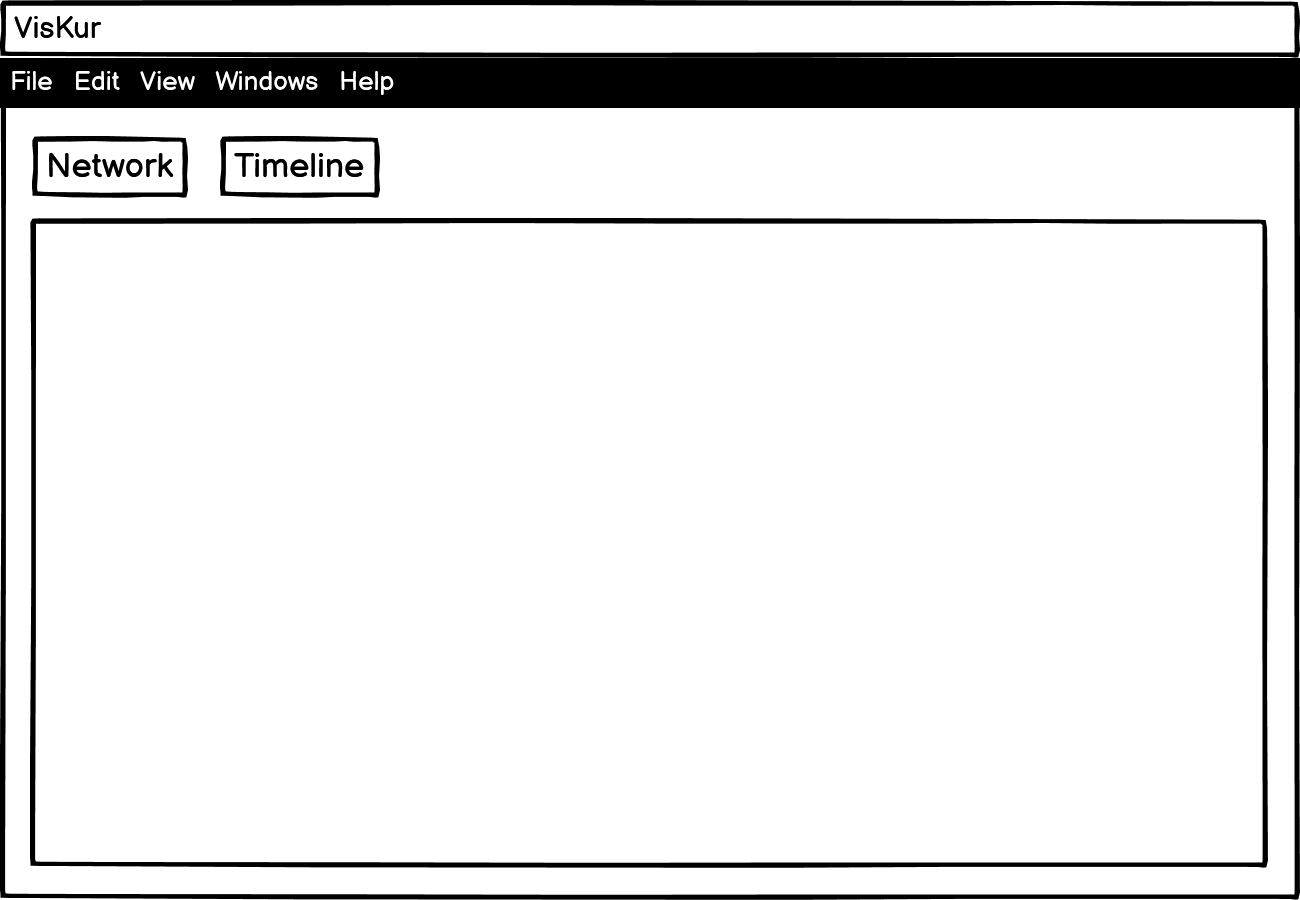
\includegraphics[width=12cm, height=8cm]{Gambar/Balsamiq.png}
    \caption{Rancangan Antarmuka Aplikasi VisKur}
    \label{fig:balsamiq}
\end{figure}
Rancangan antarmuka ini merukapan rancangan antarmuka masukan sekaligus merupakan rancangan antarmuka hasil, dimana pengguna hanya akan dapat menekan tombol \textit{Network} ataupun tombol \textit{Timeline}, dimana hasil visualisasinya akan langsung keluar pada halaman di bawahnya. Pengguna dapat melakukan pindah halaman visualisai hanya dengan menekan salah satu di antara kedua tombol tersebut. \textit{Menubar} yang berisi menu \textit{File}, \textit{Edit}, \textit{View}, \textit{Windows}, dan \textit{Help} merupakan menu bawaan dari aplikasi \textit{Electron} yang berfungsi untuk mengoperasikan aplikasi \textit{Electron} itu sendiri. 




